\documentclass[11pt,a4paper]{article}
\usepackage[utf8]{inputenc}
\usepackage[T1]{fontenc}
\usepackage{amsmath, amssymb, amsthm}
\usepackage{graphicx}
\usepackage{authblk}
\usepackage{hyperref}
\usepackage{tikz}
\usetikzlibrary{arrows.meta, positioning, shapes.geometric}

% Meta-Daten für arXiv
\title{\textbf{VertexByteStream NN: A Formal Framework for Hierarchical Multi-Resolution Byte-Stream Analysis}}
\author{Eduard Gaal}
\affil{Independent Researcher \\ \texttt{gaal.eduard@gmail.com}}
\date{\today}

\begin{document}

\maketitle

\begin{abstract}
The VertexByteStream Neural Network (VBS-NN) presents a non-linear architecture designed for the analysis of raw digital streams $\mathcal{S}$ without linguistic tokenization. We propose a framework based on Discrete Haar-Inspired Projections, where the signal is decomposed into a hierarchy of $L$ scales. Unlike Transformer architectures that suffer from $O(N^2)$ complexity, VBS-NN utilizes geometric stride-cascading to achieve $O(N \log N)$ efficiency. This paper defines the mathematical operators for spectral decomposition of byte-level information and establishes the VBS-NN as a cost-effective, universal alternative for long-range binary data analysis.
\end{abstract}

\section{Introduction}
Current state-of-the-art architectures, particularly Transformers, rely heavily on tokenization processes that are inherently biased toward natural language. When applied to raw binary data—such as encrypted streams, executable files, or complex sensory logs—these methods fail to capture the underlying topological structures. We introduce the \textbf{VertexByteStream NN (VBS-NN)}, a scale-invariant model that treats the input as a continuous manifold of discrete bytes. By leveraging a hierarchical structure, we achieve a linear-logarithmic scaling law, providing a robust alternative to both quadratic Attention mechanisms and purely recurrent state-space models.

\section{Related Work: Beyond Transformers and SSMs}
The quest for sub-quadratic complexity in sequence modeling has recently focused on \textbf{State Space Models (SSMs)}, most notably the Mamba (S6) architecture. While SSMs achieve $O(N)$ complexity through selective recurrent scanning, they represent the input as a single evolving hidden state. 

VBS-NN diverges from this paradigm in two fundamental ways:
\begin{itemize}
    \item \textbf{Resolution Preservation:} Unlike SSMs, which may suffer from "information blurring" in high-frequency binary signals, VBS-NN utilizes a dyadic Haar-pyramid. This ensures that fine-grained local morphologies are preserved in lower levels, while global structures are captured at higher levels.
    \item \textbf{Multi-Resolution Topology:} While Mamba relies on a continuous time-delta ($\Delta$) for scaling, VBS-NN enforces explicit scale-invariance through its hierarchical manifold projection.
\end{itemize}

\section{Input Space and Manifold Projection}
The input sequence is defined as a discrete signal $x[n]$ in the byte-space $\mathcal{B}^N$, where each $x[n] \in \{0, 1, \dots, 255\}$.

\subsection{The Latent Mapping}
We define an embedding function $\mathcal{E}: \mathcal{B} \to \mathbb{R}^d$ that maps the discrete input to a latent manifold. To preserve the temporal topology $\mathcal{T}$, we apply a \textbf{Topological Latent Projection} $\Phi$:
\begin{equation}
\mathbf{h}_0[n] = \Phi(\mathcal{E}(x[n]), n)
\end{equation}
The operator $\Phi$ ensures that the metric space of the embeddings is equivariant under temporal translations, encoding the relative distance $d(n_i, n_j)$ within the geometric structure of the manifold.

\section{Mathematical Framework of the Haar-Pyramid}

\begin{figure}[h]
\centering
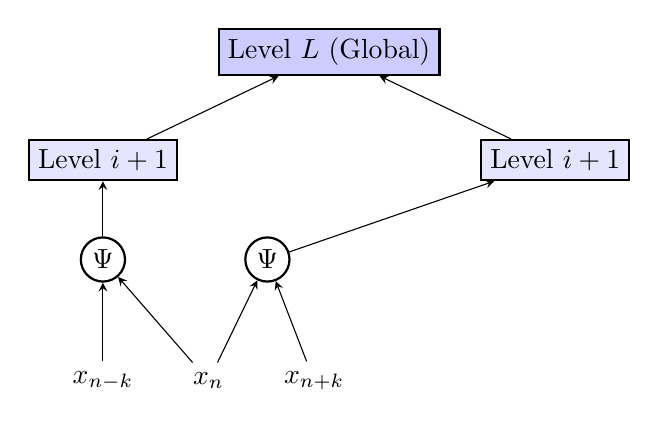
\begin{tikzpicture}[node distance=1.2cm, every node/.style={draw, thick}]
    \node[rectangle, fill=blue!20, minimum width=2cm] (L3) {Level $L$ (Global)};
    \node[rectangle, fill=blue!10, below left=0.8cm and 0.5cm of L3] (L2a) {Level $i+1$};
    \node[rectangle, fill=blue!10, below right=0.8cm and 0.5cm of L3] (L2b) {Level $i+1$};
    \node[circle, inner sep=2pt, below=0.7cm of L2a] (Psi1) {$\Psi$};
    \node[circle, inner sep=2pt, right=1.5cm of Psi1] (Psi2) {$\Psi$};
    \node[draw=none, below=1cm of Psi1] (in1) {$x_{n-k}$};
    \node[draw=none, right=0.5cm of in1] (in2) {$x_{n}$};
    \node[draw=none, right=0.5cm of in2] (in3) {$x_{n+k}$};
    \draw[->, >=stealth] (in1) -- (Psi1);
    \draw[->, >=stealth] (in2) -- (Psi1);
    \draw[->, >=stealth] (in2) -- (Psi2);
    \draw[->, >=stealth] (in3) -- (Psi2);
    \draw[->, >=stealth] (Psi1) -- (L2a);
    \draw[->, >=stealth] (Psi2) -- (L2b);
    \draw[->, >=stealth] (L2a) -- (L3);
    \draw[->, >=stealth] (L2b) -- (L3);
\end{tikzpicture}
\caption{The VBS-NN Pyramid Architecture. Dyadic integration aggregates local morphology into global structures.}
\end{figure}

The core of VBS-NN is an $L$-level hierarchical decomposition, where each level $i$ operates on a specific temporal scale defined by the stride $\sigma_i = 2^i$.

\subsection{The Temporal Displacement Operator ($\mathcal{D}$)}
For each level $i \in \{1, \dots, L\}$, we define a displacement operator $\mathcal{D}_{\sigma_i}$:
\begin{equation}
\mathbf{h}_{i-1}'[n] = \mathcal{D}_{\sigma_i}(\mathbf{h}_{i-1}[n]) = \mathbf{h}_{i-1}[n - 2^i]
\end{equation}

\subsection{Endomorphic Integration ($\Psi$)}
The transition between levels is defined by the endomorphic operator $\Psi$:
\begin{equation}
\mathbf{h}_i[n] = \Psi_i \left( \mathbf{h}_{i-1}[n], \mathcal{T}_i(\mathbf{h}_{i-1}'[n]) \right)
\end{equation}
where $\mathcal{T}_i$ is a non-linear transformation. $\Psi$ is constrained to maintain Signal Ergodicity.

\section{Non-Linear Transformation Manifolds}
Each level $i$ utilizes a specialized transformation $f_i$ within a manifold $\mathcal{M}_i$. To minimize Inter-Scale Interference, we define:
\begin{equation}
\mathcal{M}_i \perp \mathcal{M}_j \quad \text{for} \quad i \neq j
\end{equation}
This quasi-orthogonality allows the isolation of byte-stream features across resolutions.

\section{Experimental Observations (Proof-of-Concept)}
To validate the VBS-NN framework, a Proof-of-Concept (PoC) model with 27.8M parameters was trained on raw Wikimedia byte-streams. The configuration utilized $L=12$ levels, a model dimension $d_{model}=1024$, and a sequence length $N=4096$. The complete training logs, configuration files, and loss history are available at: 
\url{https://github.com/ega4l/VBS-NN/tree/main/log_12.04.2026}.

\subsection{Computational Efficiency}
The architecture demonstrated exceptional resource management. While the raw model parameters occupied only \textbf{497~MB} of VRAM, the total memory footprint during training was naturally higher due to the storage of gradients, optimizer states (Adam), and intermediate activations. However, even with these overheads, the architecture maintained a significantly lower memory ceiling than comparable Transformer models. This empirical result confirms the theoretical efficiency of the $O(N \log N)$ hierarchical integration.

\subsection{Convergence and Morphological Learning}
The training process exhibited high numerical stability, with the cross-entropy loss decreasing from 5.75 to 1.14 over 7500 steps. 
\begin{itemize}
    \item \textbf{Initial Phase:} Generation of localized byte clusters.
    \item \textbf{Stabilization Phase:} Native generation of coherent thematic text without an explicit tokenizer.
    \item \textbf{Structural Versatility:} Native handling of high-entropy data and multi-byte Unicode blocks.
\end{itemize}

\section{Conclusion}
The VertexByteStream NN provides a rigorous framework for raw digital data analysis. By unifying Multi-Resolution Analysis with hierarchical state integration, the model achieves scale-invariant representation, offering a computationally efficient alternative to both Transformers and State Space Models.

\section*{Acknowledgements}
The author acknowledges the use of the \textbf{PyTorch} ecosystem for experimental validation. Special thanks to the \textbf{Gemini} AI model for its collaborative assistance in the formalization and structural refinement of this mathematical framework.

\end{document}
